\section{Background and Related Work}
\label{sec:background}


We first discuss the communication model assumed. We then discuss LDPC codes  
and the Ising model.

\subsection{Communication model}
In a general communication system,  
a message $M$ is first encoded using an encoder into a code word $C$. This code 
word is modulated using a modulator into the signal to be sent. While being
transmitted, the signal gets affected by noise present in the channel.
The received signal is then demodulated and decoded to recover the original
message $M$, hopefully error free.

\begin{figure}[htp]
    \centerline{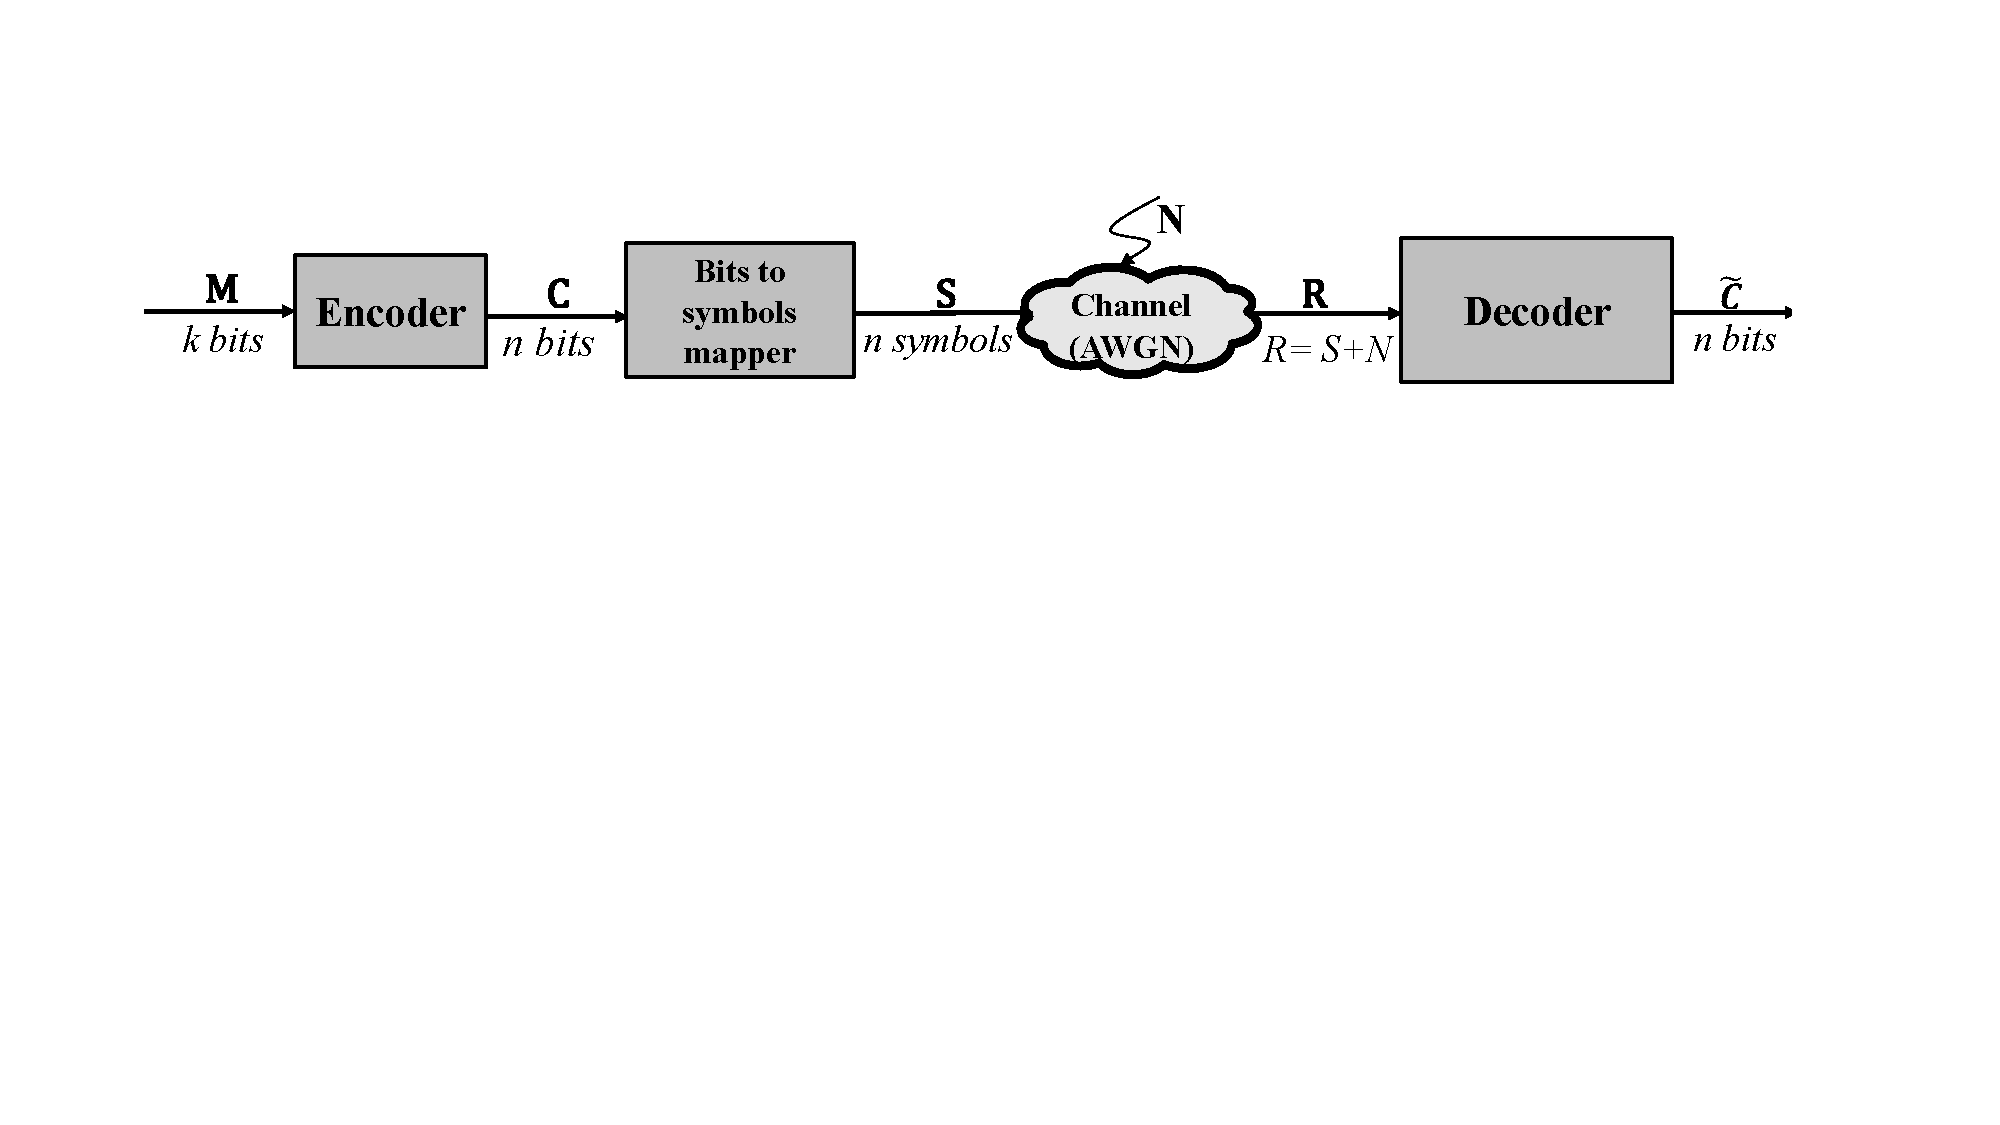
\includegraphics[width=0.50\textwidth]{FIGS/comunication_system.pdf}}
    \caption{Schematic diagram of communication system.}
    \label{fig:communication_digaram}
\end{figure}


%In this paper, we assumed a discrete communication system (Figure~\ref{fig:communication_digaram}),  where a $k$-bit binary message $M$ is  encoded into an $n$-bit code word ($C$) using a ($k$, $n$) LDPC code. This code word is modulated using the \emph{binary phase shift keying} (BPSK) modulation scheme, transmitted over a channel with additive white Gaussian noise (AWGN), and demodulated into received signal where $R_i=(1-2C_i)+\mathcal{N}(0, 1/SNR)$. 
%\todo{Professor please take a look at this paragraph }

In this paper, we assumed a discrete communication system (Fig.~\ref{fig:communication_digaram}), 
where a binary message $M$ with $k$-bit is encoded into an $n$-bit code word $C$ using a ($k$, $n$) LDPC  code. This code word is converted into an $n$-bit vector ($S_i = 1-2C_i$) of symbols representing a \emph{binary phase shift keying} (BPSK) constellation. This $n$-bit vector of symbols is transmitted over a channel with additive white Gaussian noise (AWGN). At the receiver end, we would receive a signal where $R_i=S_i+N(1/SNR)$, $N$ represents the channel's noise.


\subsection{Low Density Parity Check Codes}
LDPC codes are a class of linear block codes. The parity bits (redundant
information) are obtained using bitwise XOR operation on a selected number of
message bits. These codes are specified by a generator matrix $G_{k \times
n}$ or a parity check matrix $H_{m \times n}$, each of which can be obtained
from the other using the following relation $H\xor G^\top =0$. Here $m$ is
the number of parity bits, $n$ is the number of bits of the code word, and
$k$ is the number of bits in the message ($k=n-m$). The ratio of the length of
the message ($k$) to the size of the code word ($n$) is called the \emph{rate}: 
$r = k/n$. For example, the 5G standard uses 1/3 and 1/5 rate codes. 
The generator matrix is used for encoding a message ($M$) into a code 
word ($C$) using the following equation $C = G^\top\xor M$.
At the receiver side the decoded message is obtained from both the received
message ($R$) and the parity check matrix. The name ``low density" comes from the
sparse structure of the parity check matrix. 

\begin{figure}[htbp]
    \centering
    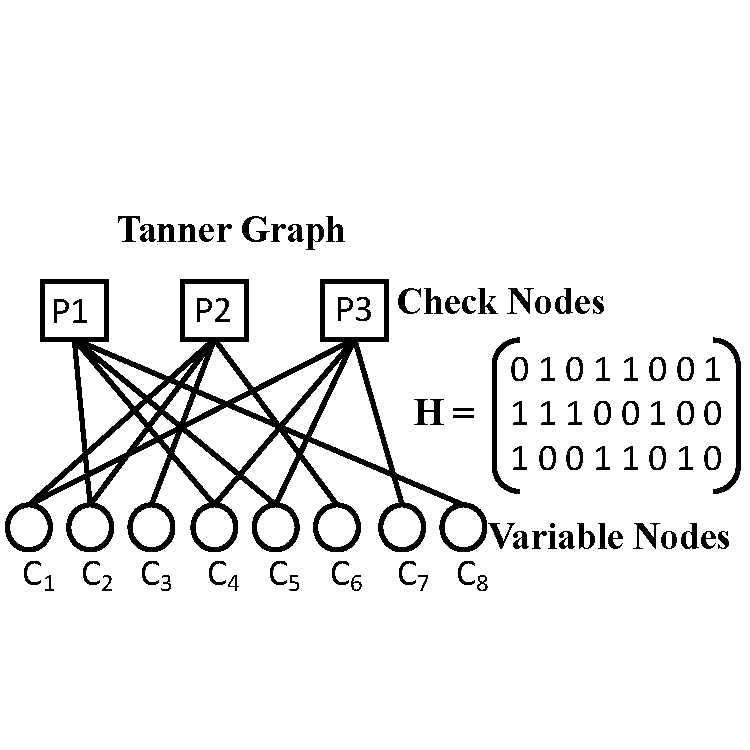
\includegraphics[width=0.38\textwidth]{FIGS/tanner_graph.pdf}
    \caption{Tanner graph with corresponding parity check matrix $H$.}
    \label{fig:tg}
\end{figure} 

LDPC codes can be represented graphically using Tanner graphs. These graphs are bipartite, meaning that the graph nodes are separated into two distinctive sets, and edges only connect nodes of two different types. The two types of nodes in a Tanner graph are variable and check nodes. Fig.~\ref{fig:tg} is an example of a Tanner graph that is constructed using parity check matrix $H$ shown above. It consists of $m$ check nodes (the number of parity bits) and $n$ variable nodes (the number of bits in an encoded message). Check node $P_i$ is connected to variable node $C_j$ if the element $h_{ij}$ of $H$ is a 1. These graphical structures are handy for analysis and decoding purposes.

%\note{I don't think the following commented paragraph is relevant.}

%There are many types of LDPC codes like regular, irregular, systematic, and nonsystematic. In regular code, the degree of rows and columns of parity check matrix are equal, i.e., the number of ones in every row is fixed. Similarly, the number of ones in every column is also fixed. In a systematic code, an encoded message is constructed with message bits followed by parity bits. The main advantage of systematic code is that the message can be directly obtained from the decoded word. The most commonly used LDPC codes are irregular systematic codes. These codes can also be constructed using a base graph as a template; hence they are called protographic~\cite{thorpe2003low}.

%\todo{fix citation above}
\begin{comment}
\subsection{Binary Phase shift Keying}
To efficiently transmit messages over communication channels, modulation schemes are employed. In this paper, we consider binary phase-shift keying (BPSK). This technique utilizes a single-frequency carrier signal and encodes digital data onto the signal by applying a phase shift. For a 0 in the data, no phase shift is applied; for a 1, the phase of the carrier signal is shifted by $180$ degrees. The data can then be recovered by the receiver by simply checking for the presence of this shift during each clock cycle by comparing it to a reference signal. If the carrier during that period has a phase shift present, the transmitted bit is decoded as 1; if not, the transmitted bit is decoded as 0.
 
Mathematically, encoding a message using BPSK modulation can be represented as follows. If $M$ is the message used for transmission, $S$ is the modulated signal, then $S = 1-2 \times M$. The received signal $R$ can be defined as $R= S+ n$, where $n$ is the noise added to the signal by the channel. 

\subsection{Decoding LDPC codes using Belief Propagation}

LDPC codes are often decoded using BP-style algorithms. The code word $\tilde{C}$ is decoded from the received message by calculating each bit's belief, or log-likelihood ratio (LLR), of being zero. 
The decoding process of LDPC code using BP is as follows: %uses tanner graph representation.
\begin{enumerate}
    \item First, the variable nodes in tanner graph are initialized using the intrinsic LLRs calculated using the received signal, and these values are broadcasted to the corresponding neighbor check nodes.
    \item Then an extrinsic LLR is calculated at each check node for each neighbor variable node based on the received LLRs from other neighbor variable nodes. Once the calculation is done, these extrinsic LLRs are again broadcasted back to each corresponding neighbor variable node.
    \item After receiving the extrinsic LLRs from the check nodes, LLRs are recalculated for each connected check node using both received extrinsic LLRs from other check nodes and the intrinsic LLR calculated from the signal.
    \item Once the calculation is done, it is broadcasted again to check nodes. This passing process is carried out until the maximum iteration count is attained or until the decoded code word can satisfy the parity check conditions.
\end{enumerate}
    This decoding methodology is also popularly known as a message-passing algorithm. There are many variants for this algorithm, like layered BP~\cite{hocevar2004reduced}, Offset Min-Sum, Normalized Min-sum~\cite{chen2005improved}, and more. These variants differ in the way they calculate the LLRs.   
    
\end{comment}

%\todo{is adjacent the same as neighboring? If so, use one to minimize confusion. Let's use "neighbor" which is simpler than "neighboring" without changing meaning.}

%\todo{make it sequential}
 \begin{comment}
 
 Let us assume the decode code word be $\tilde{C}$. Let the set of variable nodes that are connected to check node $c$ be denoted as $N(c)$, and the set of check nodes that are connected to variable node $v$ be denoted as M(v). Also $N(c)\backslash v$ and $M(v)\backslash c$ denote the set N(c) and M(v) excluding bit node v and check node c. The conventional iterative decoding process is based on the following steps:

\todo{Consistency in subscripting, and minimizing levels without ambiguity.}

%\note{A couple of ambiguities. $\tilde{c}$ is the decoded word, which means M+N bits long? But $c$ is a "node"? meaning it's not a word or related to word $\tilde{c}$, using deliberately the same letter implied some connection -- that one is a variation of the other.}

Step 1:

Each variable node $v$ is initialized using the intrinsic log-likelihood ratio  calculated by using following formula, 

\begin{equation}
    LLR_{v} = \log \frac{P(v=0/R)}{P(v=1/R)} = \frac{2R}{\sigma^2} 
\end{equation}

%\note{$0/r_i$ is still 0. Do you mean conditional probability given $r_i$}

where $\sigma$ represents the estimated variance of the Gaussian noise of the channel and $P(v=0/R)$ conditional probability of $v$ being zero, given $R$.

%\note{Do you mean estimated/assumed variance}

Step 2:

Once the LLR values are calculated at variable nodes, they are passed to the neighboring check nodes. Let $LLR_{v \rightarrow c}$ be the LLR received by the check node $c$ from variable node $v$.

At the check node $c$ for each neighboring variable node $v$, an extrinsic LLR ($LLR_{c \rightarrow v}$) is calculated  using equation~\ref{eq::llrc2v} and passed to that corresponding node.

\begin{equation}
%\begin{split}
    \label{eq::llrc2v}
    LLR_{c \rightarrow v} = 2 \times \arctanh\{   \\ \prod_{v_{i} \in N(c)\backslash v}  \frac{1+e^{-|LLR_{v_{i} \rightarrow c}|}}{1-e^{-|LLR_{v_{i} \rightarrow c } |}}\}
%    \end{split}
\end{equation}

Step 3:

After receiving the messages from the check nodes, the extrinsic messages to the neighboring check nodes are computed using equation ~\ref{eq::llrv2c} and passed to corresponding check nodes.

\begin{equation}
    \label{eq::llrv2c}
    LLR_{v \rightarrow c }  = \sum_{c_{i} \in M(v)\backslash c} LLR_{c{_i} \rightarrow v } + LLR_{v}
\end{equation}

The value of each bit of code word is decided at the variable node by calculating the final LLR by summing all LLRs received from the check nodes along with the intrinsic LLR. If the final LLR value is greater than zero, then the value of the bit is decided as zero; otherwise, 1. Step2 and Step3 are repeated until a maximum number of iterations are reached or if the decoded code word satisfies the constraint $H \xor c =\hat{0}$.

($LLR_{c \rightarrow v }$) calculated using equation~\ref{eq::llrc2v} is approximately equal to the minimum absolute value of the LLRs received from variable nodes. The sign of $LLR_{c \rightarrow v }$ is equal to the product of the sign of $LLR_{v \rightarrow c } $  all received at check node c. 

Based on this approximation, a variation of the Belief propagation called the Min-Sum algorithm was developed. The LLRs that need to be propagated to the neighbor variable node are calculated by replacing all the received LLRs with the minimum value, and the minimum value is replaced with the second minimum value. The product of the signs of received LLRs decides whether to flip the signs or not.
\end{comment}

%\todo{If this is a chapter, wouldn't this whole Ising model be described in detail somewhere earlier already? If so, this can be a very quick recall (e.g., keeping the equation), but not a repeat. Just point to the earlier chapter for detail.}
%\begin{comment}
    

\subsection{Ising Model}\label{sec:ising_mode}

The Ising model is used to describe the energy of a system of coupled
spins. The spins have one degree of freedom and take one of two values ($+1$,
$-1$). The energy of the system is a function of pair-wise coupling of the
spins ($J_{ij}$) and the interaction ($h_i$)
of some external field ($\mu$) with each
spin. The resulting energy is as follows:

\begin{equation}
\label{eqn:Ising_w_field}
% H = -\sum_{(i<j)} J_{ij}\sigma_i\sigma_j - \mu \sum_i h_i\sigma_i
E = -\sum_{\mathclap{(i<j)}} J_{ij}\sigma_i\sigma_j - \mu \sum_{\mathclap{i}} h_i\sigma_i
\end{equation}


A physical system with its energy defined by the formula naturally tends towards low-energy
states. It is as if nature tries to solve an optimization problem with
Eq.~\ref{eqn:Ising_w_field} as the objective function, which is not a trivial
task. Indeed, the cardinality of the state space grows exponentially with the
number of spins, and the optimization problem is NP-complete: it is easily
convertible to and from a generalized max-cut problem, which is part of the
original list of NP-complete problems~\cite{Karp1972}.

Thus if a physical system of spins somehow offers programmable coupling
parameters ($J_{ij}$ and $\mu h_i$ in Eq.~\ref{eqn:Ising_w_field}), they can
be used as a special purpose computer to solve\footnote{Throughout
the paper, by ``solving" an optimization problem we mean the
searching for a good solution rather than necessarily finding the global optimum, 
equivalent to reaching the ground state.} optimization problems that
can be expressed in the form of an Ising formula (Eq.~\ref{eqn:Ising_w_field}). In fact, all
problems in the Karp NP-complete set have their Ising formula
derived~\cite{lucas2014ising}. Also, if a problem already has a QUBO (quadratic
unconstrained binary optimization) formulation, mapping to Ising formula is as
easy as substituting bits for spins, \eg $\sigma_i = 2b_i-1$.

Because of the broad class of problems that can map to the Ising formula,
building nature-based computing systems that solve these problems has
attracted significant attention~\cite{kim2010quantum,berloff2017realizing,
barends2016digitized,yamaoka201520k,bunyk2014architectural,king2018observation,
bohm2019poor,hamerly2019towards,pierangeli2019large}.

\begin{comment}
Loosely speaking, an Ising machine's design goes through four
steps:
\begin{enumerate}

\item Identify the physical variable to represent a spin (be it a 
qubit~\cite{PhysRevB.82.024511}, the phase of an optical pulse~\cite{inagaki2016coherent}, 
or the polarity of a capacitor's voltage~\cite{afoakwa.hpca21}).

\item Identify the mechanism of coupling and how to program the coefficients.

\item Demonstrate the problem solving capability showing both the theory of its
operation (reveal the ``invisible hand" of nature) and satisfactory results
of practice.

\item Demonstrate superior machine metrics (solution time, energy consumption,
and construction costs).

\end{enumerate} 
\end{comment}

%It is important to note that different approaches may
%offer different fundamental tradeoffs and goes through varying gestation
%speeds. Thus it could be premature to evaluate a general approach based on
%observed instances of prototypes. Nevertheless, we provide a broad-brushed
%characterization, which can help researchers get a 
%basic sense of the landscape -- as long as the caveats are properly understood.
%\end{comment}


\begin{comment}
    

\subsection{Ising Machines}
\todo{Again, shouldn't this be present already elsewhere?}

We divide existing Ising Machines into three categories based on the technology used for their design: Quantum, Optical, and Electronic annealers. 

The latest Quantum Ising annealer manufactured by D-wave can support up to 2000 qubits~\cite{D-Wave}. The qubits are coupled to form a chimera graph. As a result of local coupling, the D-wave machine can only map up to 64 nodes all to all connected graph~\cite{hamerly2019experimental, hamerly2018scaling}. These annealers are also susceptible to noise, necessitating cryogenic operating condition that consumes much power (25KW for D-Wave 2000q)~\cite{dwave_stats}.

At the moment, the most powerful Ising machine is the Coherent Ising Machine (CIM)~\cite{inagaki2016cim, cim_yamamoto, McMahon614, 16bit_cim, ncomm_bohm2019}. It uses an optical parametric oscillator to generate and manipulate the signal to represent one spin. Unlike D-Wave, CIM nodes are all-to-all coupled. The machine has two components: an optical cavity built using kilometers of fibers, and an auxiliary computer to implement coupling between nodes. Every pulse's amplitude and phase in the optical cavity are detected, and its interaction with all other pulses is calculated using an auxiliary computer (FPGA). This computation is then used to modulate new pulses that are injected back into the optical cavity. Strictly speaking, the current implementation is a nature-simulation hybrid Ising machine. Thus, beyond the challenge of constructing the cavity, CIM  also requires a significant supporting structure that involves fast conversions between optical and electrical signals. 


 The operating principle of CIM can be viewed as a Kuramoto model~\cite{Takeda_2017},  so in theory, we can achieve a similar goal using other oscillators. This led to the design of an electronic Oscillator-based Ising Machines. These systems use LC tanks for spins and (programmable) resistors as coupling units. However, inductors are often a source of practical challenges for on-chip integration. They are area intensive and have undesirable parasitics with reduced quality and increased phase noise, which poses practical challenges in maintaining frequency uniformity and phase synchronicity between thousands of on-chip oscillators. 


Another electronic design with resistive coupling is the Bistable Resistively-coupled Ising Machine (BRIM)~\cite{afoakwa.hpca21}, in which the Ising spin is implemented as capacitor voltage controlled by a feedback circuit, making it bistable. Since it uses voltage (as opposed to phase) to represent spin, it enables a straightforward interface to implement additional architectural support for computational tasks. In BRIM, the polarity of the voltage across a capacitor represents the spin of the node and the coupling strength is inversely proportional to the resistance of the coupling resistors, i.e., $R_{ij}=\frac{R}{\abs{J_{ij}}}$, where $R$ is a scaling coefficient and the negative coupling is achieved by cross coupling the capacitors in neighboring nodes.
\end{comment}

\begin{comment}
\subsection{Existing LDPC decoders}
\todo{need to discuss about existing hardware LDPC decoders and existing Ising machines }

Most of the LDPC decoders in literature are designed by a hard-wiring a specific algorithm for a particular parity check matrix based on a chosen standard. ~\cite{?} discuss the design of LDPC decoder for 5g standard implementing offset Min-Sum Layered algorithm. The following design only supports the LDPC decoder for 5g base graph1 with an expansion factor of 384. ~\cite{?} discuss the design of the same 5g standard LDPC decoder implementing the same offset Min-sum algorithm but with support for all graphs possible in the standard. ~\cite{?} discuss pipelining the layered Min-sum algorithm for IEEE 802.e. standard to achieve high throughput.

Ising Machines have also been used for implementing decoders for LDPC codes. ~\cite{?} discuss how to convert LDPC codes into QUBO format and implement LDPC codes on D-wave. This implementation's main drawback is that it cannot fit an LDPC code of standards. This system's bit error rate (BER) is not as good as the Min-Sum algorithm's.
\end{comment}
